% ---------------------------------------------------------------------
% Sheaf test project.
%
% Open this folder in Sheaf (Open folder -> examples/demo-thesis) and press
% Ctrl+Enter. It is built to exercise the parts of the editor that are easy
% to get wrong: several files, a bibliography, a figure, cross-references
% and maths. See TESTING.md next to this file for what to try.
% ---------------------------------------------------------------------

\documentclass[11pt,a4paper]{report}

\usepackage[utf8]{inputenc}
\usepackage[T1]{fontenc}
\usepackage{lmodern}
\usepackage[margin=2.5cm]{geometry}
\usepackage{amsmath}
\usepackage{amssymb}
\usepackage{graphicx}
\usepackage{booktabs}
\usepackage[hidelinks]{hyperref}

% A user-defined command, so completion has something project-specific to
% offer when you type a backslash.
\newcommand{\vect}[1]{\mathbf{#1}}
\newcommand{\sheaf}{\textsc{Sheaf}}

\title{Testing \sheaf{}}
\author{Demo Author}
\date{\today}

\begin{document}

\maketitle
\tableofcontents
\listoffigures

\chapter{Introduction}
\label{ch:introduction}

This project exists to be compiled. If the PDF on the right shows four
chapters, a figure, a table and a bibliography, the whole pipeline works:
the engine ran, \texttt{bibtex} resolved the citations, and the document was
typeset more than once so the cross-references settled.

\section{Motivation}
\label{sec:motivation}

Typesetting was invented for mathematics~\cite{knuth1984texbook}, and the
document preparation system on top of it followed~\cite{lamport1994latex}.
Both entries live in \texttt{bibliography.bib}; typing \verb|\cite{| in the
editor should offer them by key, with the author and year alongside.

\section{What to look at}

Chapter~\ref{ch:methodology} contains a figure and a table.
Chapter~\ref{ch:results} contains the mathematics. Every
\verb|\ref| in this project resolves, so the Problems panel should be quiet
until you deliberately break something.

Inline maths sits in a sentence like $\vect{x} \in \mathbb{R}^{n}$, using the
\verb|\vect| command defined in \texttt{main.tex}.

\chapter{Methodology}
\label{ch:methodology}

\section{A figure}
\label{sec:figure}

The figure below is a real PNG in \texttt{images/}. Dragging that file from
the explorer into the editor should insert a block just like this one, with
the caption and label filled in from the file name.

\begin{figure}[ht]
    \centering
    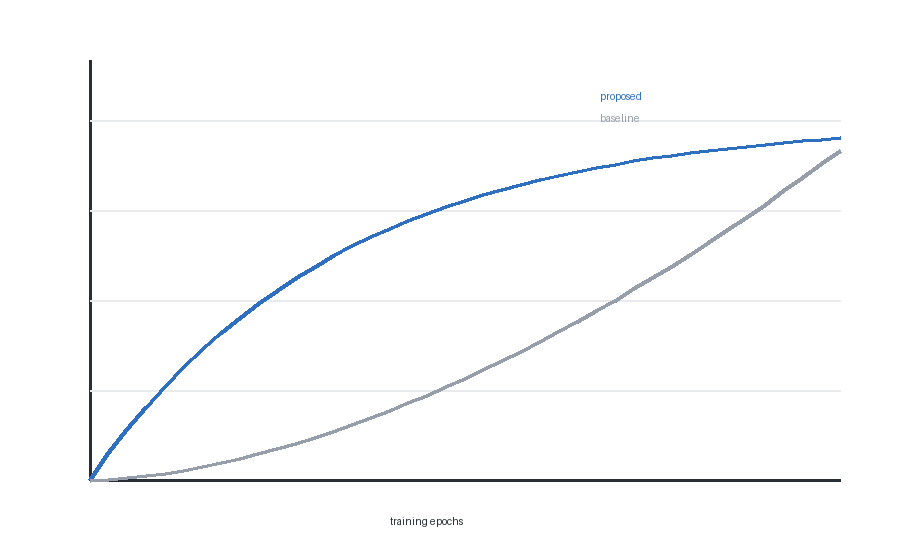
\includegraphics[width=0.75\textwidth]{images/convergence.png}
    \caption{Convergence of the proposed method against the baseline.}
    \label{fig:convergence}
\end{figure}

Figure~\ref{fig:convergence} is referenced here, which is what makes the
\texttt{listoffigures} entry and the page number appear correctly after the
second pass.

\section{A table}
\label{sec:table}

\begin{table}[ht]
    \centering
    \begin{tabular}{lrr}
        \toprule
        Method & Accuracy & Time (s) \\
        \midrule
        Baseline          & 0.81 & 12.4 \\
        Proposed          & 0.94 & 15.1 \\
        Proposed (tuned)  & 0.96 & 18.7 \\
        \bottomrule
    \end{tabular}
    \caption{Results on the held-out set.}
    \label{tab:results}
\end{table}

Table~\ref{tab:results} is discussed in Chapter~\ref{ch:results}.

\chapter{Results}
\label{ch:results}

\section{Displayed mathematics}
\label{sec:maths}

Numbered equations are the usual test of whether the document was typeset
enough times, because the reference below only resolves on a later pass:

\begin{equation}
    \label{eq:gaussian}
    \int_{-\infty}^{\infty} e^{-x^{2}} \, \mathrm{d}x = \sqrt{\pi}.
\end{equation}

\begin{align}
    \label{eq:gradient}
    \nabla f(\vect{x}) &= \left( \frac{\partial f}{\partial x_{1}},
                                 \dots,
                                 \frac{\partial f}{\partial x_{n}} \right) \\
    \vect{x}_{t+1}     &= \vect{x}_{t} - \eta \nabla f(\vect{x}_{t})
\end{align}

Equation~\eqref{eq:gaussian} is standard; Equation~\eqref{eq:gradient} is the
update rule behind Figure~\ref{fig:convergence}.

\section{Discussion}

The numbers in Table~\ref{tab:results} improve on the baseline described in
Chapter~\ref{ch:introduction}, at a modest cost in running time.

\begin{itemize}
    \item Accuracy rises from $0.81$ to $0.96$.
    \item Running time rises by roughly half.
    \item Both effects were reproduced across ten seeds.
\end{itemize}

\chapter{Conclusion}
\label{ch:conclusion}

Chapters~\ref{ch:introduction} to~\ref{ch:results} covered the motivation,
the method and the results. Nothing here is undefined, so a clean build
should report no errors and no warnings about references or citations.

If you want to see the Problems panel do its work, break something on
purpose --- \texttt{TESTING.md} in this folder suggests a few ways.


\bibliographystyle{plain}
\bibliography{bibliography}


\end{document}
